\documentclass[border=8pt]{standalone}
\usepackage[T1]{fontenc}\usepackage{lmodern}\usepackage{amsmath}\usepackage[dvipsnames]{xcolor}
\usepackage{tikz}\usetikzlibrary{positioning,arrows.meta,fit,backgrounds,calc,shapes.geometric}
% ---- colours of the system diagrams (one per MQTT topic / kind of traffic)
\definecolor{cSensor}{RGB}{37,99,235}     % sensors/<node>
\definecolor{cAlert}{RGB}{220,38,38}      % ids/alerts
\definecolor{cStats}{RGB}{22,163,74}      % ids/stats
\definecolor{cMit}{RGB}{124,58,237}       % ids/mitigation/status
\definecolor{cStatus}{RGB}{100,116,139}   % ids/status
\definecolor{cCmd}{RGB}{234,88,12}        % cmd/mitigation
\definecolor{cAttack}{RGB}{153,27,27}     % attack traffic
\definecolor{cBot}{RGB}{161,98,7}         % bot master commands (UDP, not MQTT)
\definecolor{cPi}{RGB}{220,38,90}
\definecolor{cLap}{RGB}{51,65,85}
\definecolor{cNode}{RGB}{8,145,178}
\newcommand{\topicdot}[1]{\textcolor{#1}{\rule{0.9em}{0.9em}}}

\tikzset{
  box/.style={draw=#1!70!black, fill=#1!8, rounded corners=4pt, align=center, font=\small, line width=0.7pt,
              inner sep=6pt},
  box/.default=gray,
  group/.style={draw=#1, rounded corners=8pt, line width=1.1pt, inner sep=10pt},
  grouplabel/.style={font=\bfseries\small, text=#1, fill=white, inner sep=3pt},
  pub/.style={-{Stealth[length=7pt]}, line width=1.3pt, draw=#1},
  deliver/.style={-{Stealth[length=7pt]}, line width=1.3pt, draw=#1, dashed},
  attack/.style={-{Stealth[length=8pt]}, line width=1.8pt, draw=cAttack, densely dashed},
  botcmd/.style={-{Stealth[length=7pt]}, line width=1.3pt, draw=cBot, densely dotted},
  lbl/.style={font=\scriptsize\ttfamily, text=#1, fill=white, inner sep=1.5pt},
  flow/.style={-{Stealth[length=6pt]}, line width=1pt, draw=gray!70!black},
}

\begin{document}
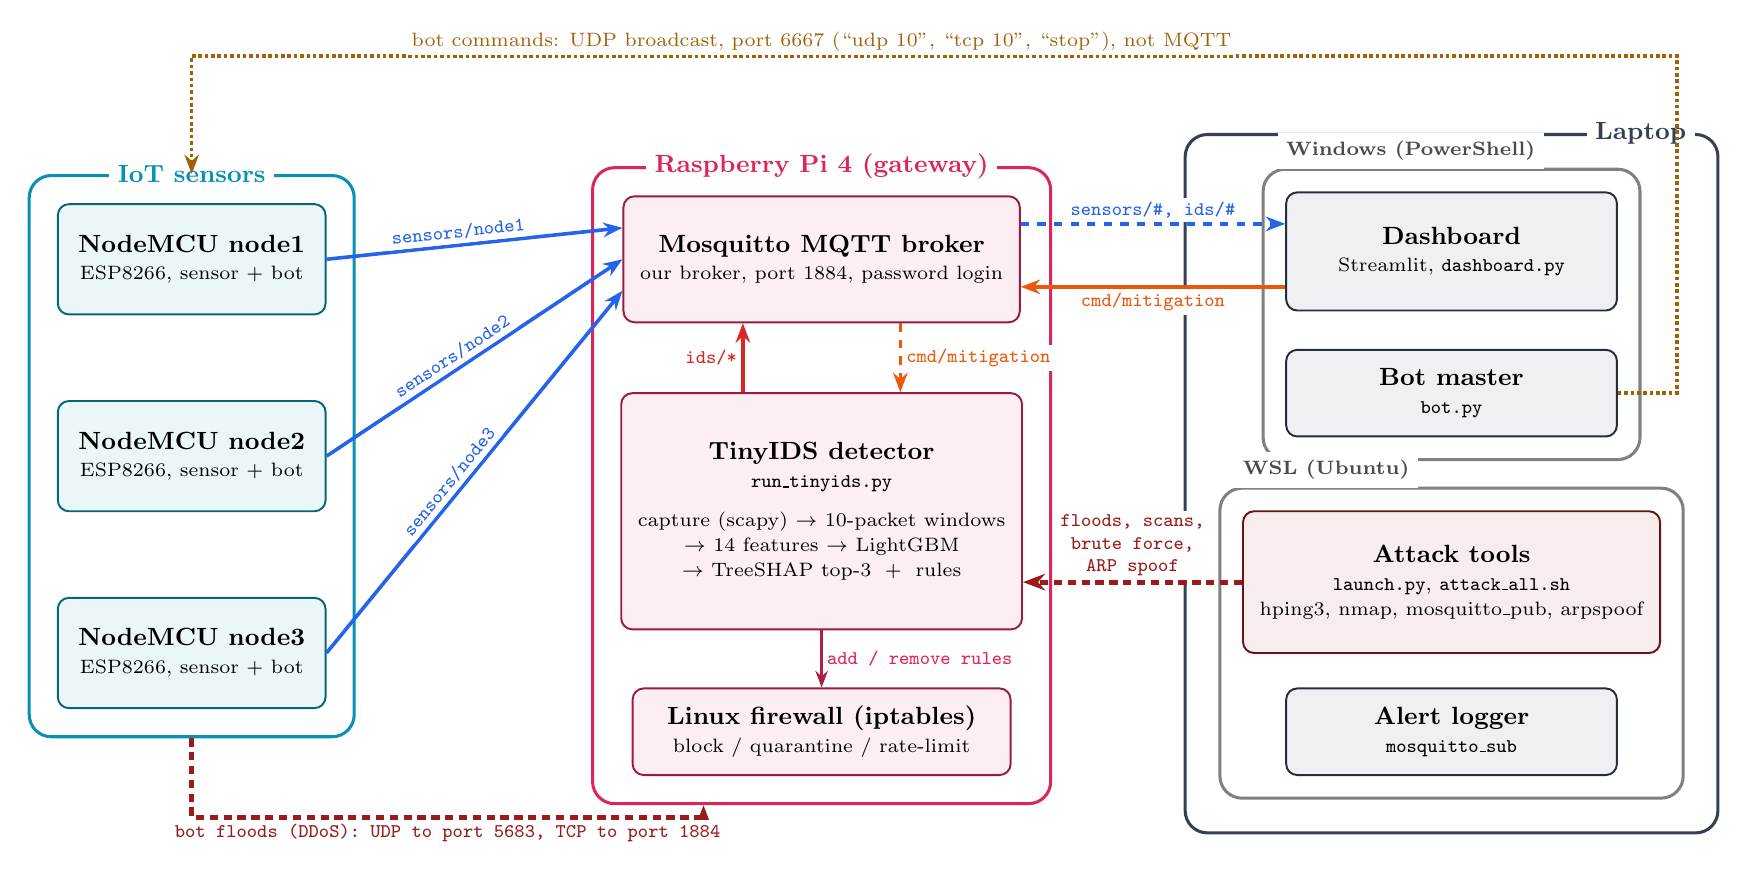
\begin{tikzpicture}[font=\small]

% ---------------- NodeMCUs
\node[box=cNode, minimum width=3.4cm, minimum height=1.4cm] (n1) at (0,3.4)
  {\textbf{NodeMCU node1}\\[-1pt]{\scriptsize ESP8266, sensor + bot}};
\node[box=cNode, minimum width=3.4cm, minimum height=1.4cm] (n2) at (0,0.9)
  {\textbf{NodeMCU node2}\\[-1pt]{\scriptsize ESP8266, sensor + bot}};
\node[box=cNode, minimum width=3.4cm, minimum height=1.4cm] (n3) at (0,-1.6)
  {\textbf{NodeMCU node3}\\[-1pt]{\scriptsize ESP8266, sensor + bot}};
\begin{scope}[on background layer]
  \node[group=cNode, fit=(n1)(n2)(n3)] (gN) {};
\end{scope}
\node[grouplabel=cNode] at (gN.north) {IoT sensors};

% ---------------- Raspberry Pi
\node[box=cPi, minimum width=4.8cm, minimum height=1.6cm] (broker) at (8,3.4)
  {\textbf{Mosquitto MQTT broker}\\[-1pt]{\scriptsize our broker, port 1884, password login}};
\node[box=cPi, minimum width=4.8cm, minimum height=3.0cm] (ids) at (8,0.2)
  {\textbf{TinyIDS detector}\\[-1pt]{\scriptsize \texttt{run\_tinyids.py}}\\[3pt]
   {\scriptsize capture (scapy) $\rightarrow$ 10-packet windows}\\[-2pt]
   {\scriptsize $\rightarrow$ 14 features $\rightarrow$ LightGBM}\\[-2pt]
   {\scriptsize $\rightarrow$ TreeSHAP top-3 \;+\; rules}};
\node[box=cPi, minimum width=4.8cm, minimum height=1.1cm] (fw) at (8,-2.6)
  {\textbf{Linux firewall (iptables)}\\[-1pt]{\scriptsize block / quarantine / rate-limit}};
\begin{scope}[on background layer]
  \node[group=cPi, fit=(broker)(ids)(fw)] (gP) {};
\end{scope}
\node[grouplabel=cPi] at (gP.north) {Raspberry Pi 4 (gateway)};

% ---------------- Laptop
\node[box=cLap, minimum width=4.2cm, minimum height=1.5cm] (dash) at (16,3.5)
  {\textbf{Dashboard}\\[-1pt]{\scriptsize Streamlit, \texttt{dashboard.py}}};
\node[box=cLap, minimum width=4.2cm, minimum height=1.1cm] (bot) at (16,1.7)
  {\textbf{Bot master}\\[-1pt]{\scriptsize \texttt{bot.py}}};
\begin{scope}[on background layer]
  \node[group=gray, fit=(dash)(bot), inner sep=8pt] (gW) {};
\end{scope}
\node[grouplabel=gray!60!black, font=\scriptsize\bfseries, anchor=south west] at ($(gW.north west)+(0.2,-0.02)$) {Windows (PowerShell)};

\node[box=cAttack, minimum width=4.2cm, minimum height=1.8cm] (atk) at (16,-0.7)
  {\textbf{Attack tools}\\[-1pt]{\scriptsize \texttt{launch.py}, \texttt{attack\_all.sh}}\\[-2pt]
   {\scriptsize hping3, nmap, mosquitto\_pub, arpspoof}};
\node[box=cLap, minimum width=4.2cm, minimum height=1.1cm] (log) at (16,-2.6)
  {\textbf{Alert logger}\\[-1pt]{\scriptsize \texttt{mosquitto\_sub}}};
\begin{scope}[on background layer]
  \node[group=gray, fit=(atk)(log), inner sep=8pt] (gL) {};
\end{scope}
\node[grouplabel=gray!60!black, font=\scriptsize\bfseries, anchor=south west] at ($(gL.north west)+(0.2,-0.02)$) {WSL (Ubuntu)};
\begin{scope}[on background layer]
  \node[group=cLap, fit=(gW)(gL), inner sep=12pt] (gLap) {};
\end{scope}
\node[grouplabel=cLap, anchor=center] at ($(gLap.north east)+(-1.0,0)$) {Laptop};

% ---------------- MQTT (solid = publish to the broker, dashed = delivered by the broker)
\draw[pub=cSensor] (n1.east) -- node[lbl=cSensor, above, sloped, pos=0.45] {sensors/node1} ($(broker.west)+(0,0.4)$);
\draw[pub=cSensor] (n2.east) -- node[lbl=cSensor, above, sloped, pos=0.45] {sensors/node2} ($(broker.west)+(0,0)$);
\draw[pub=cSensor] (n3.east) -- node[lbl=cSensor, above, sloped, pos=0.45] {sensors/node3} ($(broker.west)+(0,-0.4)$);

\draw[pub=cAlert] ($(ids.north)+(-1.0,0)$) -- node[lbl=cAlert, left] {ids/*} ($(broker.south)+(-1.0,0)$);
\draw[deliver=cCmd] ($(broker.south)+(1.0,0)$) -- node[lbl=cCmd, right] {cmd/mitigation} ($(ids.north)+(1.0,0)$);

\draw[deliver=cSensor] ($(broker.east)+(0,0.45)$) -- node[lbl=cSensor, above] {sensors/\#, ids/\#} ($(broker.east -| dash.west)+(0,0.45)$);
\draw[pub=cCmd] ($(broker.east -| dash.west)+(0,-0.35)$) -- node[lbl=cCmd, below] {cmd/mitigation} ($(broker.east)+(0,-0.35)$);

% ---------------- attacks and bot commands
\draw[attack] (atk.west) -- node[lbl=cAttack, above, align=center] {floods, scans,\\brute force,\\ARP spoof} (atk.west -| ids.east);
\draw[attack] (gN.south) -- ++(0,-1.0) -| node[lbl=cAttack, below, pos=0.25] {bot floods (DDoS): UDP to port 5683, TCP to port 1884} ($(gP.south)+(-1.5,0)$);
\draw[botcmd] (bot.east) -- ++(0.75,0) |- ($(gN.north)+(0,1.5)$) -- (gN.north);
\node[lbl=cBot, font=\scriptsize, above] at ($(gN.north)+(8,1.5)$) {bot commands: UDP broadcast, port 6667 (``udp 10'', ``tcp 10'', ``stop''), not MQTT};
\draw[flow, draw=cPi!80!black] (ids.south) -- node[lbl=cPi, right] {add / remove rules} (fw.north);

\end{tikzpicture}
\end{document}
